%%%%%%%%%%%%%%%%%%%%%%%%%%%%%%%%%%%%%%%%%
% Structured General Purpose Assignment
% LaTeX Template
%
% This template has been downloaded from:
% http://www.latextemplates.com
%
% Original author:
% Ted Pavlic (http://www.tedpavlic.com)
%
% Note:
% The \lipsum[#] commands throughout this template generate dummy text
% to fill the template out. These commands should all be removed when 
% writing assignment content.
%
%%%%%%%%%%%%%%%%%%%%%%%%%%%%%%%%%%%%%%%%%

%----------------------------------------------------------------------------------------
%   PACKAGES AND OTHER DOCUMENT CONFIGURATIONS
%----------------------------------------------------------------------------------------

\documentclass{article}

\usepackage{fancyhdr} % Required for custom headers
\usepackage{lastpage} % Required to determine the last page for the footer
\usepackage{extramarks} % Required for headers and footers
\usepackage{graphicx} % Required to insert images
\usepackage{lipsum} % Used for inserting dummy 'Lorem ipsum' text into the template
\usepackage{amsmath}
\usepackage{xcolor}
\usepackage{listings}
\usepackage[toc,page]{appendix}
\usepackage{algorithm}
\usepackage{algorithmic}

% Margins
\topmargin=-0.45in
\evensidemargin=0in
\oddsidemargin=0in
\textwidth=6.5in
\textheight=9.0in
\headsep=0.25in 

\linespread{1.1} % Line spacing

% Set up the header and footer
\pagestyle{fancy}
\lhead{\hmwkAuthorName} % Top left header
\chead{\hmwkClass\ (\hmwkClassInstructor): \hmwkTitle} % Top center header
\rhead{\firstxmark} % Top right header
\lfoot{\lastxmark} % Bottom left footer
\cfoot{} % Bottom center footer
\rfoot{Page\ \thepage\ of\ \pageref{LastPage}} % Bottom right footer
\renewcommand\headrulewidth{0.4pt} % Size of the header rule
\renewcommand\footrulewidth{0.4pt} % Size of the footer rule

\setlength\parindent{0pt} % Removes all indentation from paragraphs

%----------------------------------------------------------------------------------------
%   DOCUMENT STRUCTURE COMMANDS
%   Skip this unless you know what you're doing
%----------------------------------------------------------------------------------------

% Header and footer for when a page split occurs within a problem environment
\newcommand{\enterProblemHeader}[1]{
    \nobreak\extramarks{#1}{#1 continued on next page\ldots}\nobreak
    \nobreak\extramarks{#1 (continued)}{#1 continued on next page\ldots}\nobreak
}

% Header and footer for when a page split occurs between problem environments
\newcommand{\exitProblemHeader}[1]{
    \nobreak\extramarks{#1 (continued)}{#1 continued on next page\ldots}\nobreak
    \nobreak\extramarks{#1}{}\nobreak
}

\setcounter{secnumdepth}{0} % Removes default section numbers
\newcounter{homeworkProblemCounter} % Creates a counter to keep track of the number of problems
\setcounter{homeworkProblemCounter}{0}

\newcommand{\homeworkProblemName}{}
\newenvironment{homeworkProblem}[1][Problem \arabic{homeworkProblemCounter}]{ % Makes a new environment called homeworkProblem which takes 1 argument (custom name) but the default is "Problem #"
    \stepcounter{homeworkProblemCounter} % Increase counter for number of
% problems
    \renewcommand{\homeworkProblemName}{#1} % Assign \homeworkProblemName the
% name of the problem
    \section{\homeworkProblemName} % Make a section in the document with the
% custom problem count
    \enterProblemHeader{\homeworkProblemName} % Header and footer within the
% environment
}{
    \exitProblemHeader{\homeworkProblemName} % Header and footer after the
% environment
}

\newcommand{\problemAnswer}[1]{ % Defines the problem answer command with the content as the only argument
    \noindent\textbf{\emph{Answer: }}#1 % Just put a keyword Answer in
    % bold/italic at the beginning
}

\newcommand{\homeworkSectionName}{}
\newenvironment{homeworkSection}[1]{ % New environment for sections within homework problems, takes 1 argument - the name of the section
    \renewcommand{\homeworkSectionName}{#1} % Assign \homeworkSectionName to the
% name of the section from the environment argument
    \subsection{\homeworkSectionName} % Make a subsection with the custom name
% of the subsection
    \enterProblemHeader{\homeworkProblemName\ [\homeworkSectionName]} % Header
% and footer within the environment
}{
    \enterProblemHeader{\homeworkProblemName} % Header and footer after the
% environment
}

\newtheorem{theorem}{Theorem}[homeworkProblemCounter]
\newtheorem{lemma}[theorem]{Lemma}
\newtheorem{proposition}[theorem]{Proposition}
\newtheorem{corollary}[theorem]{Corollary}

\newenvironment{proof}[1][Proof]{
    \begin{trivlist}
        \item[\hskip \labelsep {\bfseries #1}]
    }{
        \end{trivlist}
}
\newenvironment{definition}[1][Definition]{
    \begin{trivlist}
        \item[\hskip \labelsep {\bfseries #1}]
    }{
        \end{trivlist}
}
\newenvironment{example}[1][Example]{
    \begin{trivlist}
        \item[\hskip \labelsep {\bfseries #1}]
    }{
        \end{trivlist}
    }
\newenvironment{remark}[1][Remark]{
    \begin{trivlist}
        \item[\hskip \labelsep {\bfseries #1}]
    }{
        \end{trivlist}
}

\newcommand{\qed}{
    \nobreak \ifvmode \relax \else
    \ifdim\lastskip<1.5em \hskip-\lastskip
    \hskip1.5em plus0em minus0.5em \fi \nobreak
    \vrule height0.75em width0.5em depth0.25em\fi
}

\lstset{
    frame=single,
    breaklines=true,
    postbreak=\raisebox{0ex}[0ex][0ex]{\ensuremath{\color{red}\hookrightarrow\space}}
}
   
%----------------------------------------------------------------------------------------
%   NAME AND CLASS SECTION
%----------------------------------------------------------------------------------------

\newcommand{\hmwkTitle}{Assignment\ \#7} % Assignment title
\newcommand{\hmwkDueDate}{Thursday,March\ 12,\ 2015} % Due date
\newcommand{\hmwkClass}{ECS\ 222A} % Course/class
\newcommand{\hmwkClassTime}{TR 4:40pm-6:00pm} % Class/lecture time
\newcommand{\hmwkClassInstructor}{Daniel Gusfield} % Teacher/lecturer
\newcommand{\hmwkAuthorName}{Wenhao Wu} % Your name

%----------------------------------------------------------------------------------------
%   TITLE PAGE
%----------------------------------------------------------------------------------------

\title{
    \vspace{2in}
    \textmd{\textbf{\hmwkClass:\ \hmwkTitle}}\\
    \normalsize\vspace{0.1in}\small{Due\ on\ \hmwkDueDate}\\
    \vspace{0.1in}\large{\textit{\hmwkClassInstructor\ \hmwkClassTime}}
    \vspace{3in}
}

\author{\textbf{\hmwkAuthorName}}
\date{} % Insert date here if you want it to appear below your name

%----------------------------------------------------------------------------------------

\begin{document}

    \maketitle
    
    %----------------------------------------------------------------------------------------
    %   TABLE OF CONTENTS
    %----------------------------------------------------------------------------------------
    
    %\setcounter{tocdepth}{1} % Uncomment this line if you don't want subsections listed in the ToC
    
    \newpage
    \tableofcontents
    \newpage

    %----------------------------------------------------------------------------------------
    %   PROBLEM 1
    %----------------------------------------------------------------------------------------
    \begin{homeworkProblem}
        In class on thursday, we talked about the factor of two approximation
        algorithm for minimum-size node cover problem in an undirected graph
        $G$: find a maximal Independent Set of edges of $G$, call it $M$ , then
        form $A(G)$ by taking both ends of each edge in $M$. $A(G)$ is a node
        cover, and we proved that its size is at most twice the size of $O(G)$,
        where $O(G)$ is a minimum-size node cover of $G$. That is,
        $|A(G)|/|O(G)| \leq 2$. In class, I said that we can find a subset
        $A'(G)$ of $A(G)$ (possibly equal), which is also a node cover of $G$,
        such that $|A'(G)|/|O(G)| < 2$. More precisely, we have the following:
        \begin{quotation}
            Claim: Either some node $x$ can be removed from $A(G)$ so that
            $A'(G) = A(G)-\{x\}$ is a node cover of $G$, or $A(G)$ is a
            minimum-size node cover.
        \end{quotation}
        Prove the claim, and show how it establishes the better ratio. As a
        hint, examine two cases: either there is a node $v$ in $A(G)$ such that
        for every edge $(u, v)$ in $G$, $u$ is also in $A(G)$; or there is no
        such node. To handle the latter case, extend the proof we gave in class
        that $|A(G)|/|O(G)| \leq 2$.
            
        \vspace{10pt}
        \problemAnswer{
            \begin{lemma}
                \label{lemma:1_1}
                If $|A(G)|/|O(G)| = 2$, then for any optimal node cover $O(G)$,
                for any edge $(u, v)\in M$ we must have either $u\in O(G)$ and
                $v\notin O(G)$, or $v\in O(G)$ and $u\notin O(G)$. Consequently,
                $O(G)\subset A(G)$.
            \end{lemma}
            \begin{proof}
                If $|A(G)|/|O(G)| = 2$, we have $|M| = |O(G)|$. Given an optimal
                node cover $O(G)$ and an edge $(u, v)\in M$:
                \begin{itemize}
                    \item If $u\notin O(G)$ and $v\notin O(G)$, then edge $(u,
                    v)$ is not covered by $O(G)$, this contradicts with the fact
                    that $O(G)$ is a node cover.
                    \item If $u\in O(G)$ and $v\in O(G)$, since $|M| = |O(G)|$,
                    according to Pigeonhole principle, there must be another
                    edge $(u', v')\in M$ such that $u'\notin O(G)$ and $v'\notin
                    O(G)$. This again contradicts with the fact that $O(G)$ is a
                    node cover.
                \end{itemize}
                Consequently, for any edge $(u, v)\in M$ we must have either $u\in O(G)$ and
                $v\notin O(G)$, or $v\in O(G)$ and $u\notin O(G)$. Since there
                are exactly $|O(G)|$ edges in $M$, we have $O(G)\subset A(G)$.
            \end{proof}
            
            \begin{lemma}     
                \label{lemma:1_2}
                If $|A(G)|/|O(G)| = 2$, then for any edge $(u, v) \in M$, there
                is no pair of nodes $u'$, $v'$ (possibly $u'=v'$) such that
                $(u, u')\in G$ and $(v, v')\in G$. In other words, for any edge
                in the independent set $M$, it is impossible that both end nodes
                are adjacent to some other nodes.
            \end{lemma}
            \begin{proof}
                Assume for contradiction that there exists edge $(u, v) \in M$
                and $u'$, $v'$ such that $(u, u')\in G$ and $(v, v')\in G$.
                Since $M$ is an independent set, $u'\notin A(G)$ and $v'\notin
                A(G)$. According to Lemma~\ref{lemma:1_1}, without loss of
                generality we can assume that $u\in O(G)$ and $v\notin
                O(G)$. Since $O(G)\subset A(G)$, $v'\notin A(G)$ indicates that
                $v'\notin O(G)$. Consequently, we have found an edge $(v,
                v')\in G$ not covered by $O(G)$. This contradicts with the fact
                that $O(G)$ is a node cover. The lemma is proved.
            \end{proof}
            
            \begin{corollary}
                If $|A(G)|/|O(G)| = 2$, we can find some node $x\in A(G)$ such
                that $A(G)-\{x\}$ is also a node cover.
            \end{corollary}
            \begin{proof}
                According to Lemma~\ref{lemma:1_2}, we can find $(u, v)\in M$
                such that $v$ is not adjacent to any node in $G$ other than $u$.
                Consequently, $A(G)-\{v\}$ is also a node cover.
            \end{proof}
            Now we have proved that we can always find a node cover $A(G)$ such
            that $|A(G)|/|O(G)| < 2$. Note that the original claim is
            wrong. A counter example is shown in Fig~\ref{fig:1_1}. $M =
            \{(2,3), (4,5)\}$ is a maximal independent set. However, no node can
            be removed from $A(G) = \{2, 3, 4, 5\}$ so that $A'(G)$ is still a
            node cover, yet $A(G)$ is not a minimum-size node cover since we
            have one $O(G) = \{1, 2, 4\}$.
            
            \begin{figure}[!h]
                \centering
                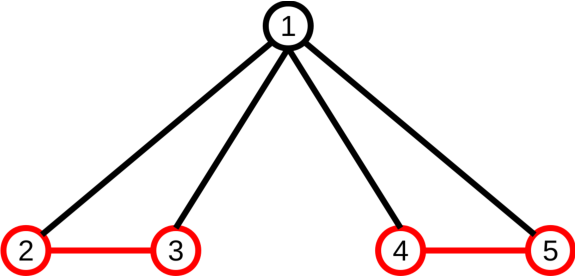
\includegraphics[width=0.3\columnwidth]{figs/1_1.pdf}
                \caption{$M = \{(2,3), (4,5)\}$, $A(G) = \{2, 3, 4, 5\}$,
                $|O(G)| = 3$ and $O(G)$ must contains node $1$.}
                \label{fig:1_1}
            \end{figure}
            
        }
        
    \end{homeworkProblem}
    
    %----------------------------------------------------------------------------------------
    %   PROBLEM 2
    %----------------------------------------------------------------------------------------
    \begin{homeworkProblem}
        In class we stated that the Satifiability problem is NP-complete, that
        the Independent Set problem is NP-complete and the Node-Cover Problem is
        NP-complete. So in this problem you may assume those problems, but only
        those problems, are known to be NP-complete.

        \begin{homeworkSection}{\homeworkProblemName(a)}
            In a problem we call the ZZZ problem, the input is a number $k$, and
            bipartite graph $G$, where the two node sets on the two sides of $G$
            are denoted $A$ and $B$. The answer to an instance of problem ZZZ is
            yes if and only if there is a subset $S$ of size at most $k$ of the
            nodes in $A$, such that every node in $B$ is adjacent to at least
            one node in $S$. Prove that problem ZZZ is NP-complete.
            
            \vspace{10pt}
            \problemAnswer{
                Firstly, if the answer to problem ZZZ is ``yes'', there exists a
                subset $S\subset A$ of size at most $k$ (certificate) which can
                be verified in $O(|V|^2)$ time that every vertex in $B$ is
                adjacent to at at least one vertex in $S$. And if the answer to
                problem ZZZ is ``no'', no certificate can trick the verification
                into saying ``yes''. Consequently, ZZZ problem is NP.
                
                An instance $(G, k)$ for a Node-Cover problem, i.e.
                whether there is a node cover $C$ of size at most $k$ in graph
                $G = (V, E)$, can be reduced into an instance of ZZZ problem as
                follows. For the bipartite graph $H$, define $A = V$, $B = \{uv
                | (u, v)\in E\}$, i.e. $A$ contains the same node as $G$ and for
                each edge in $G$ a node is added to $B$. The edge set $F$ of $H$
                is defined as $F=\{(u, uv), (v, uv)|(u, v) \in E\}$, i.e. for
                any edge $(u, v)$ in $G$, define 2 edges $(u, uv)$ and $(v, uv)$
                in $H$ where $uv \in B$ is the node corresponding to the edge
                $(u, v)$.
                
                \begin{lemma}
                    \label{lemma:2a_1}
                    The answer to instance $(G, k)$ of Node-Cover problem is
                    ``yes'' iff the answer to instance $(H, k)$ of ZZZ
                    problem is ``yes''.
                \end{lemma}
                \begin{proof}
                    Suppose $S$ is a node cover in $G$, we claim
                    that every node in $B$ is adjacent to at least one node in
                    $S\subset A$. To see this, suppose for contradiction that
                    there exists a node $uv \in B$ that is not adjacent to any
                    node in $S$, then there exists two nodes $u\in A\backslash
                    S$, $v\in A\backslash S$ such that $(u, v) \in E$.
                    Consequently, we find an edge in $G$ that is not covered by
                    $S$, which contradicts with the fact that $S$ is a node
                    cover. As a result, the answer to instance $(H, k)$ of ZZZ
                    problem is ``yes'' if the answer to instance $(G, k)$ of
                    Node-Cover problem is ``yes''.
                    
                    On the other hand, suppose in bipartite graph $H$ there
                    is $S\in A$ such that every node in $B$ is adjacent to some
                    node in $S$, we claim $S$ is also a node cover in $G$. To
                    see this, suppose for contradiction that $S$ is not a node
                    cover in $G$, i.e. there exists $(u, v)\in E$ such that
                    $u\notin S$ and $v\notin S$. In bipartite graph $H$,
                    consider node $uv \in B$. From the construction of $H$, $uv$
                    is adjacent to only $u$ and $v$, therefore $uv$is not
                    adjacent to any node in $S$. This contracdits with the
                    assumption. As a result, the answer to instance $(G, k)$ of
                    Node-Cover problem is ``yes'' if the answer to instance $(H,
                    k)$ of ZZZ problem is ``yes''.
                \end{proof}
            
                Since we assume Node-Cover problem to be NP-complete, from
                Lemma~\ref{lemma:2a_1} we know that ZZZ problem is NP-hard.
                Since ZZZ problem is also NP, we conclude that ZZZ problem is
                NP-complete.
                
            }
        \end{homeworkSection}
        
        \begin{homeworkSection}{\homeworkProblemName(b)}
            In a problem we call the QQQ problem, the input is an undirected
            graph $G = (V, E)$ and an undirected graph $G_1$. There are no node
            or edge labels. The answer to an instance of problem QQQ is yes if
            and only if there is an ``induced'' subgraph $G' = (V', E')$ of $G$
            which is isomorphic (indentical in this context) to $G_1$. In an
            induced subgraph containing the set of nodes $V'$, the edge set $E'$
            consists of \emph{every} edge whose two endpoints are both in $V'$.
            Prove that Problem QQQ is NP-complete.
             
            \vspace{10pt}
            \problemAnswer{
                Firstly, if the answer to problem QQQ is ``yes'', there exists
                an induced subgraph $G'$ of $G$ which is isomorphic to $G_1$.
                Define the certificate as $G'$ and the correspondence between
                nodes in $G'$ and $G_1$, the correctness of $G'$ can be verified
                in  $O(|V|^2)$ time. And if the answer to problem QQQ is ``no'',
                no certificate can trick the verification into saying ``yes''.
                Consequently, QQQ problem is NP.
                
                An instance $(G, k)$ of the independent set problem, i.e.
                whether there is an independent set of edges $S$ of size at
                most $k$ in graph $G = (V, E)$, can be reduced into a QQQ
                problem instance $(G, G_1)$, where $G_1 = (V_1, E_1)$. We define
                $V_1 = \{x_1, \ldots, x_k, y_1, \ldots, y_k\}$ and $E_1 =
                \{(x_1, y_1),\ldots, (x_k, y_k)\}$. Apparently, an independent
                set of size $k$ corresponds to an induced subgraph isomorphic to
                $G_1$. Consequently, the answer to instance $(G, k)$ of
                independent set problem is ``yes'' iff the answer to instance
                $(G, G_1)$ of QQQ problem is ``yes''.
                
                Since we assume Independent Set problem to be NP-complete, from
                the above reduction we know that QQQ problem is NP-hard.
                Since QQQ problem is also NP, we conclude that QQQ problem is
                NP-complete.
            }
        \end{homeworkSection}
        

    \end{homeworkProblem}
    
    %----------------------------------------------------------------------------------------
    %   PROBLEM 3
    %----------------------------------------------------------------------------------------
    \begin{homeworkProblem}
        In an undirected, connected graph $G$, a subset $S$ of nodes of $G$ is
        called a \emph{Dominating Set} if every node in $G$ is adjacent to at
        least one node in $S$. Note that a Dominating Set is not the same as a
        Node Cover. The Dominating Set Problem has input $(G, k)$. The answer to
        an instance of the Dominating Set problem is yes, if and only if $G$ has
        a Dominating Set of size at most $k$.
        
        The following idea shows how to reduce any instance of the Node Cover
        Problem, when the input graph is connected, to an Instance of the
        Dominating Set Problem. Note that the Node Cover problem is NP-complete
        even when the restricted to the case where the input graph is required
        to be connected.
        
        Given an instance $(H, t)$ of the Node Cover Problem ($H$ is a
        connected, undirected graph, and $t$ is the target), create a new
        graph $G$ consisting of $H$ plus one new node $uv$ for each edge $(u,
        v)$ in $H$. Node $uv$ in $G$ has an edge to node $u$ in $G$ and an edge
        to node $v$ in $G$. So each edge $(u, v)$ in $H$ is associated with a
        triangle in $G$ consisting of nodes $u$, $v$, $uv$. It helps to draw a
        picture. Then the input to the Dominating Set Problem is $(G, k)$, where
        $k = t$.
        
        Prove that $H$ has a Node Cover of size at most $t$ if and only if $G$
        has a Dominating Set of size at most $t$. Hint: establish first that a
        smallest Dominating Set of $G$ can be found using only the original
        nodes in $H$.
        
        \vspace{10pt}
        \problemAnswer{
            Firstly we establish a smallest Dominating Set of $G$ can be found
            using only the original nodes in $H$.
            
            \begin{lemma}
                \label{lemma:3_1}
                If $S$ is a dominating set in $G$, then for each edge $(u, v)$
                in $H$, at least one of $u, v$ is in $S$.
            \end{lemma}
            \begin{proof}
                Suppose for contradiction that there exists a dominating set
                $S$ and an edge $(u, v)$ in $H$ such that $u\notin S$ and
                $v\notin S$. According to the construction of $G$, node $uv$ is
                adjacent to only 2 two nodes $u$ and $v$, consequently, $uv$ is
                not adjacent to any node in $S$. This contradicts with the fact that
                $S$ is a dominating set. Consequently, we conlude that at least
                one of $u, v$ is in $S$.
            \end{proof}
            
            \begin{lemma}
                \label{lemma:3_2}
                For a dominating set $S$. The following procedure results in a
                dominating set $S'$ containing only the original nodes in $H$:
                Initialize $S'=S$. For any node $uv \in S$
                \begin{itemize}
                    \item If $uv, v$ in $S$, replace $uv$ with $u$ in $S'$.
                    \item If $uv, u$ in $S$, replace $uv$ with $v$ in $S'$.
                \end{itemize}
                (From Lemma~\ref{lemma:3_1} these are the only 2 possible
                scenarios.) Apparently, the number of nodes in $S'$ is equal to
                or less than that in $S$.
            \end{lemma}
            \begin{proof}
                To see that $S'$ is also a dominating set, for any node $x\in
                G$, since $S$ is a dominating set, we have $x$ must be adjacent
                to some node $y\in S$.
                \begin{itemize}
                    \item If $y\in H$, i.e. $y$ is an original node in $H$, then
                    $y\in S'$. Consequently, node $x$ is still adjacent to some
                    node in $S'$.
                    \item If $y = uv$ corresponds to some edge $(u, v)$ in $H$,
                    then we have either $x=u$ or $x=v$. Since both $u$ and $v$
                    are in $S'$, $x$ must be adjacent to some node in $S'$.
                \end{itemize}
                Consequently, $S'$ is also a dominating set.
            \end{proof}
            \begin{corollary}
                \label{corollary:3_3}
                A smallest Dominating Set of $G$ can be found using only the
                original nodes in $H$.
            \end{corollary}
            \begin{proof}
                From Lemma~\ref{lemma:3_2}, suppose $S$ is a smallest Dominating
                Set, we can always construct a dominating set $S'$ no larger
                than $S$ that contains only the original nodes in $H$.
            \end{proof}
            
            Now we are ready to show that $H$ has a Node Cover of size at most
            $t$ if and only if $G$ has a Dominating Set of size at most $t$.
            \begin{itemize}
                \item If $G$ has a dominating set $S$ of size $t$, from
                Corollary~\ref{corollary:3_3} $G$ has a dominating set $S'$ of
                size $t'\leq t$ contains only the original nodes in $H$. We
                claim that $S'$ is a node cover in $H$. Assume for contradiction
                that there exists an edge $(u, v)$ in $H$ such that $u\notin
                S'$ and $v\notin S'$, then node $uv \in G$ is not adjacent to
                any node in $S'$ since $uv$ is adjacent only to $u$ and $v$.
                This contradicts with the assumption that $S$ is a dominating
                set in $G$. Consequently, $S'$ is a node cover in $H$ of size at
                most $t$.
                \item If $H$ has a node cover $S$ of size $t$, we claim that $S$
                is also a dominating set in $G$. To see this, given $x\in G$,
                we show that either $x\in S$ or $x$ is adjacent to some node in
                $S$:
                \begin{itemize}
                    \item If $x = uv$ corresponds to some edge $(u, v)$ in $H$,
                    then edge $(u, v)$ must be covered by $S$ in $H$, therefore
                    either $u\in S$ or $v\in S$. Since $uv$ is adjacent to both
                    $u$ and $v$, $uv$ is adjacent to at least one node in $S$.
                    \item If $x = u$ corresponds to an original node in $H$, we
                    have either $u\in S$ or $u\notin S$. In the latter case,
                    since $H$ is connected, there exists node $v$ such that edge
                    $(u, v)$ is in $H$, thus covered by $S$. Then $u\notin S$
                    indicates that $v\in S$, therefore $u$ is adjacent to some
                    node in $S$.
                \end{itemize}
                Consequently, $S$ is a dominating set of size $t$ in $G$.
            \end{itemize}
            In conclusion, $H$ has a Node Cover of size at most $t$ if and only
            if $G$ has a Dominating Set of size at most $t$.
        }
        
    \end{homeworkProblem}
    %\clearpage
    
   
    
    %----------------------------------------------------------------------------------------

\end{document}